\graphicspath{ {./figures/} }
\section{Experiments \label{experiments}}
	In this section, we present experimental results, including the environment, software  and data sets used to obtain these results.
    \subsection{Computational Environment}
    All the code used to build the DL models we have presented in this paper was written in Python 3.8. We build these models  using Tensorflow 2.4, Keras 2.4, and Jupyter Notebooks to aid with the visualization. 
    We trained the models on  a Dell PowerEdge R940XA Server that had 2 Intel Xeon Gold 5122 processors, 256GB of RAM, 2 NVIDIA Tesla V100 32G Passive GPU, and a 2TB HDD. Only one Tesla V100 GPU was allocated to us for training the models. On this server, we ran our software on a Docker container running atop the Ubuntu 18.04 LTS operating system. 
    
%        \begin{itemize}
%            \item Python 3.8 was the language used for developing the machine learning models. 
%            \item The libraries used to implement the models were Tensorflow 2.4, Keras 2.4, and Jupyter Notebook to help with the visualization.
%            \item The models were trained on a Dell Poweredge R940XA Server that had 2 Intel Xeon Gold 5122 processors, 256GB of RAM, 2 NVIDIA Tesla V100 32G Passive GPU, and a 2TB HDD.
%            \item The server ran a Docker container with the Ubuntu 18.04.4 LTS OS.
%        \end{itemize}
    \subsection{Datasets}
    All the data used to train and test the models were obtained from the PubChem database. We used the PubChem REST API to capture
    a data set with  $\sim$1.33 million entries. These entries were randomly chosen from the database. For our training and testing, we  then randomly 
	chose 600,000 entries. Each entry contained the following information: CID (the unique identifier used by PubChem), molecular formula, canonical SMILES, isometric SMILES, molecular weight, XLogP, exact mass, TPSA, and complexity.
	
	We used the the canonical SMILES  representation for training all the models, including for the molecular fragments in the third model as well.
	The canonical SMILES was preferred since it gave us enough information about the molecular structure and helped ensure that each compound had a unique SMILES string. It also was a simpler representation to work with. Recall that since the SMILES consisted of the symbols of the elements and special characters with no white-space, instead of sentences, we considered more effective to tokenize the strings at the character level before being given then as input to the model. 
	
	To generate the fragments we used the RDKit \cite{rdkit} Python library, and we use  the RECAP algorithm. 
	 After being generated, the fragments for a molecule  were stored as a string where each fragment was separated by a white-space.
	Most of the SMILES strings had a length of less than 200 characters, with the average length being around 56 characters. But a few of them had length of 1000 characters of more. Most of the fragments generated also had a length of less than 200, with an average length of 144 characters. 
	
	The molecular weight and XLogP of the compounds were also important elements as they were necessary to establish how good predictions of the models were.The molecular weights in the dataset ranged from $\sim$1 to $\sim$10,000 g/mol, with the average being at $\sim$439.44 g/mol.
The XLogP in the dataset ranged from $\sim$-70 to $\sim$161, with the average being at $\sim$4.58.
	
	   The training set consisted of 600,000 elements of the data and was used for training the model.
             The validation set consisted of 200,000 elements of the data and was used while training to help fit the hyperparameters of the model.
             Finally, the test set consisted of 200,000 elements of the data was used to evaluated the model after training.
            
            
%        \begin{itemize}
%            \item The data used for training the models were obtained from the PubChem database (REF).
%            \item Using the PubChem REST API we were able to generate a dataset of $\sim$1.33 million entries.
%            \item These entries were randomly chosen from the database. For our training and testing, we  then randmly 
%            \item Each entry contained the following information: CID (the unique identifier used by PubChem), molecular formula, canonical SMILES, isometric SMILES, molecular weight, XLogP, exact mass, TPSA, complexity.
%            \item We used the the canonical SMILES  representation for training all the models, including for the molecular fragments in the third model as well.
%            \item The canonical SMILES was preferred since it gave us enough information about the molecular structure and helped ensure that each compound had a unique SMILES string.
%            \item Most of the SMILES strings had a length of less than 200, with the average length being around 56.
%            \item Since the SMILES consisted of the symbols of the elements and special characters with no white-space, instead of sentences, we considered more effective to tokenize the strings at character level before being given as input to the model. 
%            \item It was then converted into a vector and given padding to ensure they all had the same length.
%            \item The fragments used as input were generated using the RECAP technique.
%            \item Fragments are similar to SMILES string, but instead represent the compound as a set of smaller SMILES strings.
%            \item To generate the fragments we used the RDKit \cite{rdkit} Python library.
%            \item When generated they were stored as a string where each fragment was separated by a white-space.
%            \item Since not all of the compounds generated a set of fragments, then when not available the SMILES string was used instead. Acting as a single fragment.
%            \item Most of the fragments generated also had a length of less than 200, with an average length of 144 characters. 
%            \item These fragment strings were processed the same way as the SMILES strings.
%            \item They were tokenized at a character level, vectorized, and given a padding.
%            \item The molecular weight and XLogP of the compounds were also important as they were necessary to establish how good predictions of the models were.
%            \item The molecular weights from the dataset ranged from $\sim$1 to $\sim$10,000 g/mol, with the average being at $\sim$439.44 g/mol.
%            \item The XLogP from the dataset ranged from $\sim$-70 to $\sim$161, with the average being at $\sim$4.58.
%            \item The dataset was split into 3 subsets: training, validation, and test sets. 
%            \item The training set consisted of 600,000 elements of the data and was used for training the model.
%            \item The validation set consisted of 200,000 elements of the data and was used while training to help fit the hyperparameters of the model.
%            \item Finally, the test set consisted of 200,000 elements of the data was used to evaluated the model after training.
%            \item The data that was not used was saved for any further testing we might want to do on the model.
%        \end{itemize}
    % Not sure what to call this section
    \subsection{Training the Models}
    \begin{itemize}
        \item The first model implemented was the one for predicting the molecular weight of a compound.
        \item Initially the padding used for the input data was 300, but was later changed to 1000 since this better accommodated for some of the much longer SMILES strings present in the dataset.
        \item The results of this model, shown in Figures \ref{fig:model2-mol-weight-loss} and \ref{fig:model2-mol-weight-predictions}, were promising and as a result we proceeded to tune it.
        \item To tune the model we used the Python library Talos (REF), which permitted us to tune various hyperparameters.
        \item Some of the initial hyperparameters tuned were: learning rate, epochs, and batch size. \item Later more parameters were included like the amount of units per layer and the kernel size in the convolutional layers.
        \item Our main metric for comparison was the resulting validation loss of the models.
        \item The overall best model is the one described in section \ref{archi}, which gave us the results shown in Figures \ref{fig:model20-mol-weight-loss} and \ref{fig:model20-mol-weight-predictions}.
        \item It was noted, based on the various models trained, that there was a tendency for the models to give good predictions for smaller molecular weights, but as the molecular weight got larger so did the error.
        \item This was likely the result of the distribution of the data as very little of the data was larger than 2,000 g/mol.
        \item Due to this a few models were trained using only data within 0 and 2,000 g/mol, to see if we could get more precise results in this limited range.
        \item The results of the best out of those models can be seen in Figures \ref{fig:model23-mol-weight-loss} and \ref{fig:model23-mol-weight-predictions}
        \item Using the architecture of the molecular weight model as a guide we proceeded to develop the next two model for predicting the XLogP value.
        \item The first XLogP model followed the same architecture as the previous, but was tuned so it would be more suited for prediction XLogP, hence why their architecture are so similar.
        \item The results of this model can be seen in Figures \ref{fig:model7-xlogp-loss} and \ref{fig:model7-xlogp-predictions}.
        \item Finally, the model which receives as input both SMILES and fragments was implemented similar to the previous model, but with the adjustments needed for the additional input.
        \item This last model gave us the results shown in Figures \ref{fig:frag2-xlogp-loss} and \ref{fig:frag2-xlogp-predictions}.
    \end{itemize}
    
    % Figures
    % Initial molecular weight model results
    \begin{figure}
        \centering
        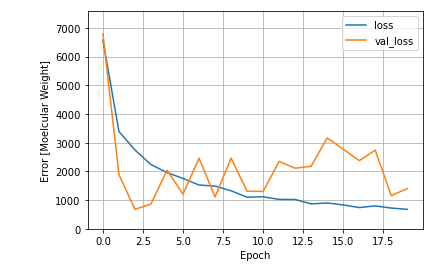
\includegraphics[width=0.5\textwidth]{loss_gragh_20_epoch.PNG}
        \caption{The loss graph of the first trained model for predicting molecular weight.}
        \label{fig:model2-mol-weight-loss}
    \end{figure}
    \begin{figure}
        \centering
        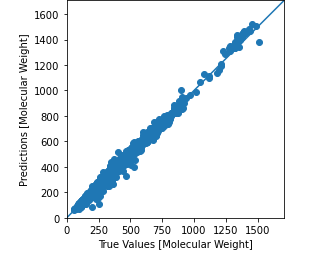
\includegraphics[width=0.5\textwidth]{model_2_prediction.PNG}
        \caption{Results of the first trained model for predicting molecular weight.}
        \label{fig:model2-mol-weight-predictions}
    \end{figure}
    
    % Best molecular weight model results
    \begin{figure}
        \centering
        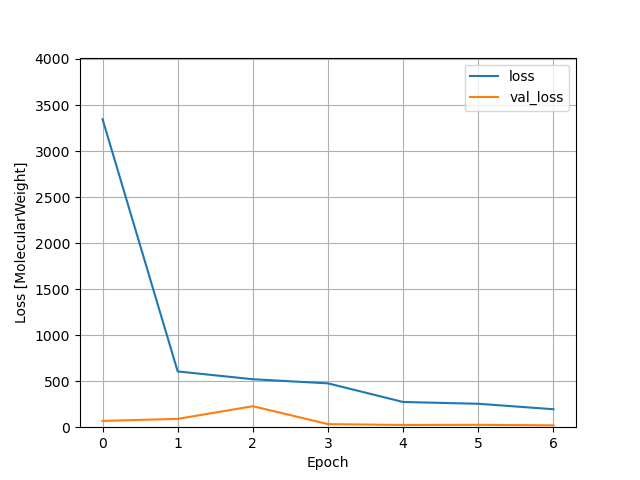
\includegraphics[width=0.5\textwidth]{model_20_7_epochs_loss_MolecularWeight.png}
        \caption{Loss graph of the best overall tuned model for predicting molecular weight.}
        \label{fig:model20-mol-weight-loss}
    \end{figure}
    \begin{figure}
        \centering
        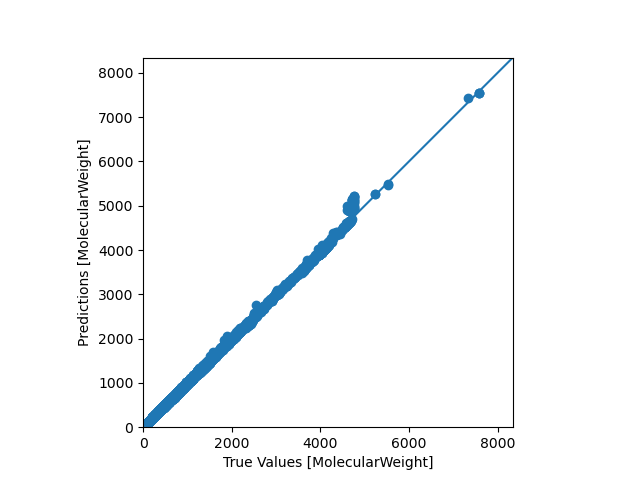
\includegraphics[width=0.5\textwidth]{model_20_7_epochs_predictions_MolecularWeight.png}
        \caption{Results of the best overall tuned model for predicting molecular weight.}
        \label{fig:model20-mol-weight-predictions}
    \end{figure}
    
    % Best molecular weight < 2000 model results
    \begin{figure}
        \centering
        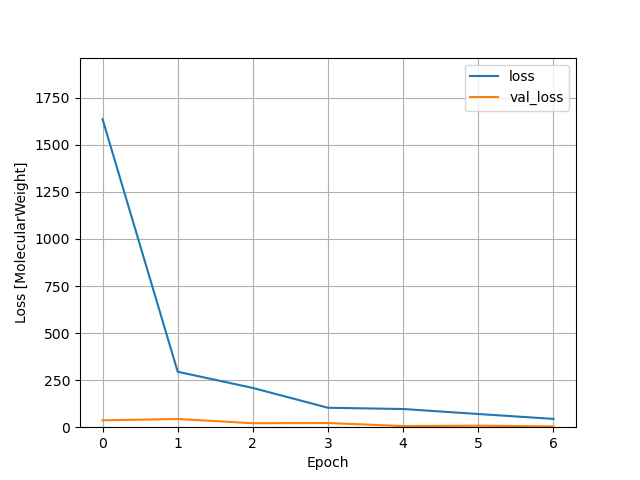
\includegraphics[width=0.5\textwidth]{model_23_7_epochs_loss_MolecularWeight.png}
        \caption{Loss graph of the best tuned model for predicting molecular weights smaller than 2,000.}
        \label{fig:model23-mol-weight-loss}
    \end{figure}
    \begin{figure}
        \centering
        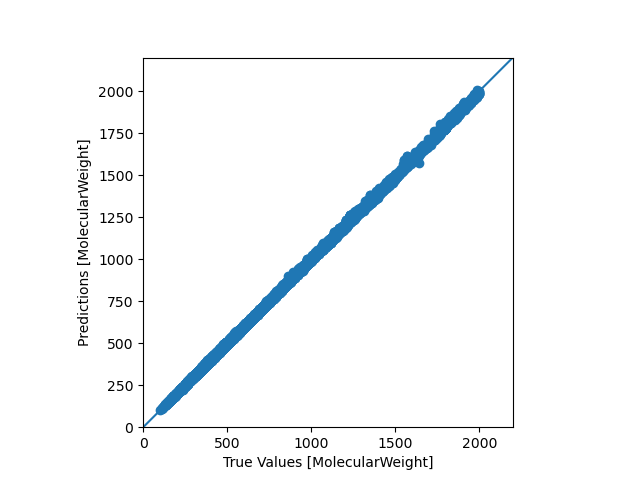
\includegraphics[width=0.5\textwidth]{model_23_7_epochs_predictions_MolecularWeight.png}
        \caption{Results of the best tuned model for predicting molecular weights smaller than 2,000.}
        \label{fig:model23-mol-weight-predictions}
    \end{figure}
    
    % Best XLogP model results
    \begin{figure}
        \centering
        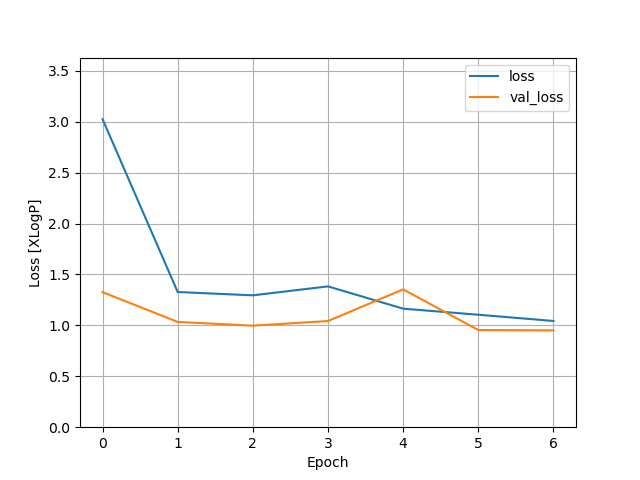
\includegraphics[width=0.5\textwidth]{model_7_7_epochs_loss_XLogP.png}
        \caption{Loss graph of the model trained for predicting XLogP.}
        \label{fig:model7-xlogp-loss}
    \end{figure}
    \begin{figure}
        \centering
        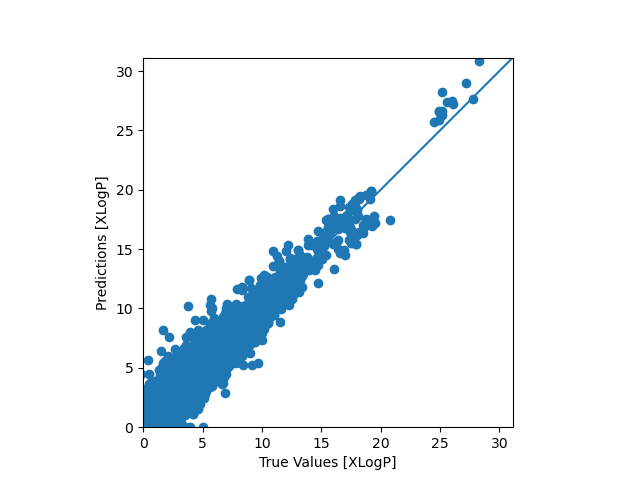
\includegraphics[width=0.5\textwidth]{model_7_7_epochs_predictions_XLogP.png}
        \caption{Results of the model trained for predicting XLogP.}
        \label{fig:model7-xlogp-predictions}
    \end{figure}
    
    % Fragment XLogP model results
    \begin{figure}
        \centering
        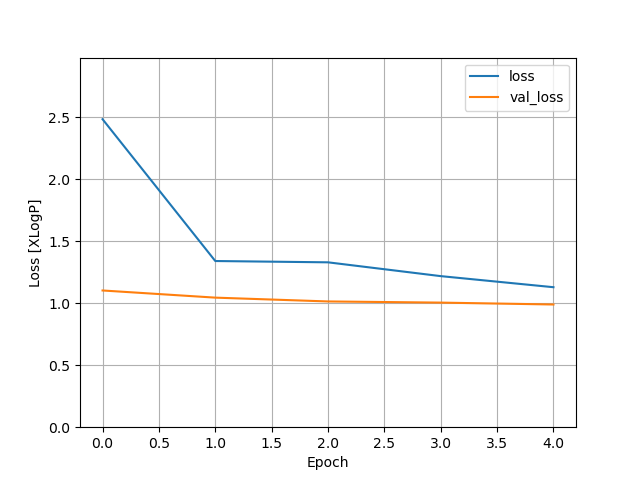
\includegraphics[width=0.5\textwidth]{figures/XLogP_model_2_5_epochs_loss.png}
        \caption{Loss graph of the model that used SMILES and fragments as input for predicting XLogP.}
        \label{fig:frag2-xlogp-loss}
    \end{figure}
    \begin{figure}
        \centering
        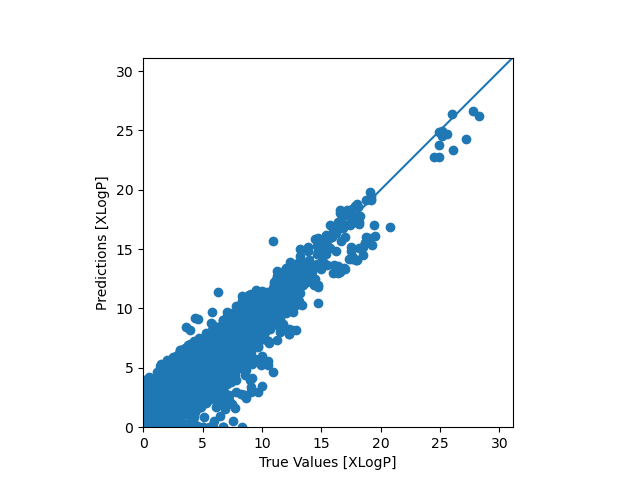
\includegraphics[width=0.5\textwidth]{figures/XLogP_model_2_5_epochs_predictions.png}
        \caption{Results of the model that used SMILES and fragments as input for predicting XLogP.}
        \label{fig:frag2-xlogp-predictions}
    \end{figure}
    
    \subsection{Results}
    \begin{itemize}
        \item The graphs shown in Figures \ref{fig:model2-mol-weight-predictions}, \ref{fig:model20-mol-weight-predictions}, and \ref{fig:model23-mol-weight-predictions}, show the results of the three molecular weight models after receiving the 200,000 sample test set as input.
        \item It can be observed that the second and third model had more precise predictions compared to the original as their prediction were closer to the center line that represents the true value.
        \item It can also be noted from Figures \ref{fig:model20-mol-weight-loss} and \ref{fig:model23-mol-weight-loss} that not many epochs are needed for training the models since the training loss dips quickly and the validation loss tends to stay low during training.
        \item To have a better idea how the newer models compared to the original we gave each model a small test set as input, the results obtained are in Figure \ref{fig:comparison_mol_weight}.
        \item The new test set consisted of 500 SMILES that the models had not seen before and the expected molecular weight values were under 2,000 g/mol.
        \item It can be noted that the two newer models did better at predicting the molecular weight closer to their true value, with the second model giving the best results with a MSE of 37.527.
        \item The third model although was trained specifically for compounds with molecular weights below 2,000 g/mol still did worse than the second model, this suggests that limiting training to a subset of the data does not help enhance performance.
        \item Additionally we also compared the two architectures that predict the XLogP value.
        \item When comparing how both models did with the validation set, Figures \ref{fig:model7-xlogp-predictions} and \ref{fig:frag2-xlogp-predictions}, it can be noted that the results were similar. 
        \item The first model was slightly more centered on its predictions, while the second leaned more towards predicting lower than the expected value. 
        \item The behaviour can be better appreciated in Figure \ref{fig:comparison_xlog} where we compare both models on a new test set, similar to how we did with the molecular weight models.
        \item The models were also given a small test set of 500 new SMILES and for the second model included its fragments.
        \item The model whose input is exclusively SMILES string performed much better with a MSE of 1.996 compared to the 17.083 from the other. 
        \item It becomes clear that the model trained using fragments does not do well with large XLogP values.
        \item As we can see in its graph in Figure \ref{fig:comparison_xlogp} most predictions are clustered together close to the origin of the graph and the largest prediction given is close to 10.
        \item It should also be noted that when training the XLogP models the validation loss stayed at best close to 1, barely getting lower than that, this can be observed in Figures \ref{fig:model7-xlogp-loss} and \ref{fig:frag2-xlogp-loss}.
        \item One additional observation of the models developed is that they do not tend to do well on short SMILES strings. 
        \item This can be observed in Figures \ref{fig:comparison_mol_weight1} and \ref{fig:comparison_xlogp1}, where the models were tested using another test set of 500 SMILES string, this time the strings were limited to having between 5 to 20 characters.
        \item For all the models the results were more sporadic.
        \item In the case of the molecular weight models the second model seems to have a limit at around 100 g/mol, it does not seem capable of giving a value lower.
        \item Regardless it still performed better than the other two, but not by a large margin as in the previous dataset.
        \item For the XLogP models the first graph is more sporadic while the other concentrates at the bottom, further showing that this model likes to predict below the true value. 
        
    \end{itemize}
    % Figures
    % Comparison between all the molecular weight models on new data
    \begin{figure}
        \centering
        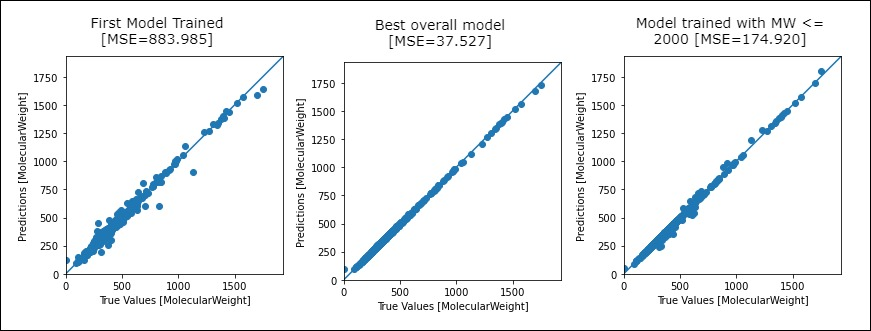
\includegraphics[width=0.5\textwidth]{figures/graphs-Mol-Wei_Comp1.jpg}
        \caption{Comparing results of the three models that predict the molecular.}
        \label{fig:comparison_mol_weight}
    \end{figure}
    \begin{figure}
        \centering
        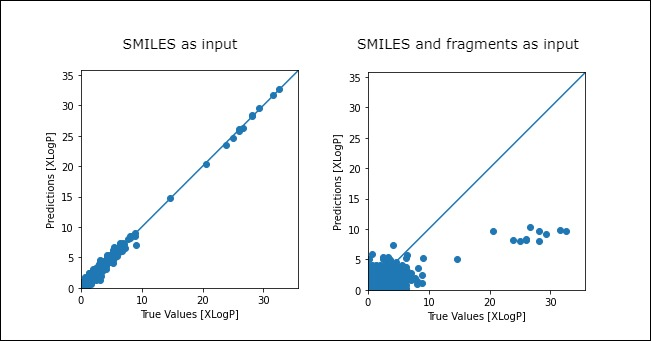
\includegraphics[width=0.5\textwidth]{figures/graphs-XLog_Comp1.jpg}
        \caption{Comparing results of the two XLogP architectures implemented.}
        \label{fig:comparison_xlogp}
    \end{figure}
    \begin{figure}
        \centering
        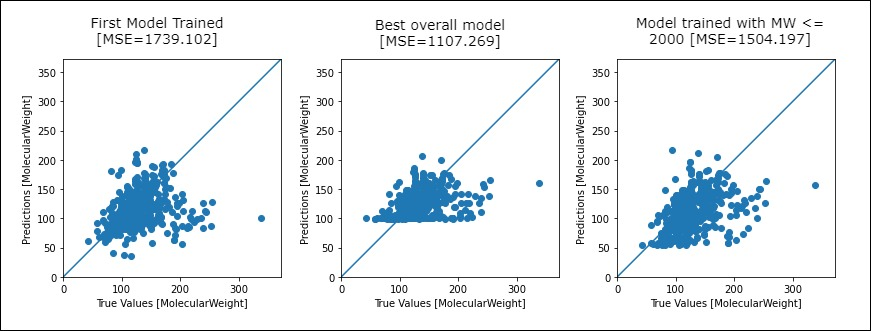
\includegraphics[width=0.5\textwidth]{figures/graphs-Mol-Wei_Comp2.jpg}
        \caption{Comparing results of the three models that predict the molecular on SMILES string between 5 - 20 characters}
        \label{fig:comparison_mol_weight1}
    \end{figure}
    \begin{figure}
        \centering
        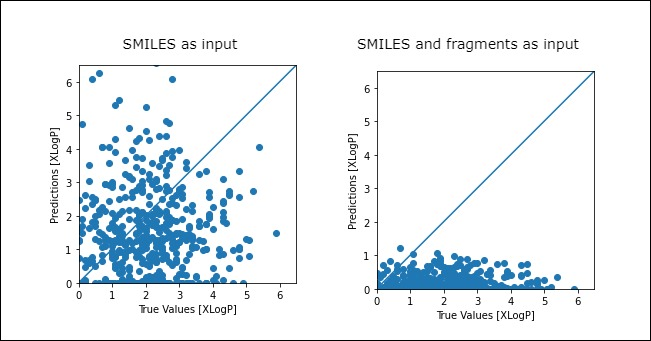
\includegraphics[width=0.5\textwidth]{figures/graphs-XLog_Comp2.jpg}
        \caption{Comparing results of the two XLogP architectures implemented on SMILES string between 5 - 20 characters.}
        \label{fig:comparison_xlogp1}
    \end{figure}